\documentclass[a4paper,oneside,12pt]{book}

% #f7efe3

\usepackage[margin=.75in]{geometry}
\usepackage[english]{babel}
\usepackage{microtype}
\usepackage{enumerate}
\usepackage{listings}
\usepackage{hyperref}
\usepackage{graphicx}
\usepackage{float}
\usepackage{blindtext}
\usepackage{color}

\definecolor{lg}{rgb}{.97,.97,.97}
\lstset{
    breaklines=true,
    backgroundcolor=\color{lg},
    captionpos=b,
}



\title{ECL: Basic Programming}
\author{Atreya Bain - 1RV18CS030}
\begin{document}
\maketitle{}%
\tableofcontents
\
\pagebreak

\chapter{Introduction}

ECL is a declarative language that can be used to work with huge data projects, in the HPCC platform. Its most powerful feature is that you can re-use each query for every subsequent queries. Here's a sample program (It is part of the ECL Playground sample code).

So, breaking it down, there are two types of ECL Code: Definitions, which define what is to be done (eg. loading up a dataset, sorting through a part of a file, and so on) and actions, which are, well, actions; they define what are the actions that are required. Here's a sample program that is from the ECL Playground (most likely the first thing you will see when you load up the playground):

\lstinputlisting[caption={Comments, Definitions, and Actions},firstline=5]{../source/00-eclStarter.ecl}

The first thing to keep in mind, is that ECL, is \textbf{case-insensitive}. Comments are done in a C/C++ fashion of \lstinline!//! as line-comments and \lstinline!/* */! as block comments. It uses the standard \lstinline!object.property! structure and can be use to nest definitions neatly (Note that it is not an object oriented language).

Execution in ECL, is done by following the trail given by the actions. The execution of an action, requires definitions, which are compiled and executed accordingly. Note that this implies that there \textbf{may not be} an explicit execution order; execution is reordered in a way that helps speed up execution.

Consider the example above, it consists of three definitions, one record, one dataset, and one last definition which is a filter of the previous dataset.
The final line is an action which creates the execution graph. (Execution graph? Huh?)

\section{Graph Solver}

ECL can actually be considered an optimized graph solver. Digging into ECL Watch, we can obtain this pretty (simple) graph for that previous code sample:
\begin{figure}[h]
    \centering
    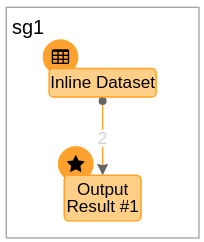
\includegraphics[width=.4\linewidth]{../media/simplegraph}
    \caption{Graph}
\end{figure}

Each node is some activity, and the (computation) graph is solved in the best possibly way in ECL. The fact that the computation can be very well optimized by mentioning "what" to do, rather than "how" to do, presents a lot of speedups and the ability to parallelize the program as much as possible.

Look at this other example, for which the source code is given:

\lstinputlisting[caption={Source code for the graph below (Don't worry about what's in the code)},firstline=2]{../source/01-graph2.ecl}

\begin{figure}[h]
    \centering
    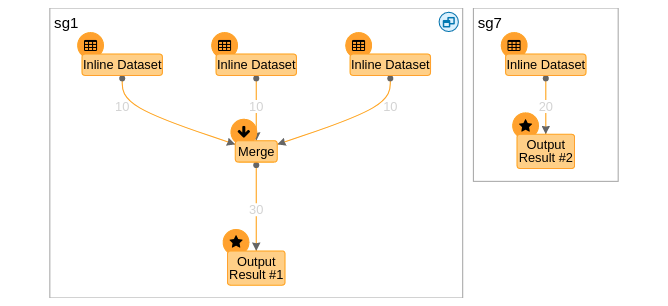
\includegraphics[width=.7\linewidth]{../media/bitlesssimplegraph.png}
    \caption{Bit less simple graph}
\end{figure}

The program above, has two outputs (actions). In this case, two graphs are generated and can be executed accordingly. This mindset of "graphs" is rather important to the understanding of ECL, as this will help differentiate it from the traditional imperative style of programming.

\section{A rundown of the chapters}

The other chapters give examples in ECL, their outputs, and (hopefully) a good understanding of how they work. The last chapter, gives some key methodologies in ECL that is necessary/useful for Machine Learning.

Datasets used have been provided, and can be referred to from the provided repository \url{https://github.com/chrisvrose/bda6-ecl-basics}. Record structures will be given as per the examples.

There are 4 datasets of importance to note:
\begin{enumerate}
    \item heart\_failure.csv - A dataset having 13 attributes of a patient, and whether they have heart disease or not. Refer to the \href{https://www.kaggle.com/ronitf/heart-disease-uci}{kaggle page} for more data. 
    \item house\_prices\_data.csv - A dataset that shows the price of a house, given key attributes about it. Refer to the \href{https://www.kaggle.com/shivachandel/kc-house-data}{user's submission on kaggle} for more data.
    \item Salary\_Data.csv - Years of Experience vs Salary. Its the smallest dataset, and undoubtedly the simplest
    \item Social\_Network\_Ads.csv - Similar to the earlier dataset, but includes some additional attributes.
\end{enumerate}

The scope expected in the programs given below is `~eclbasics', but the reader is free to configure them accordingly.

\chapter{Basics}

\section{Data Types \& Beginner Steps in ECL}

ECL has a list of basic data types, but more may be created by the developer.
Some common datatypes are enumerated below. (Use this for quick reference)
\begin{table}[h]
\centering
\begin{tabular}{|c|c|}\hline
Data Type & What it's about \\\hline\hline
STRING[n] & Packed (or null-terminated) string \\\hline
UTF8 & Unicode character string \\\hline
UNICODE[\_locale][n] &  UTF-16 encoded unicode character string \\\hline
INTEGER[n] & n-byte integer value n can be: 1 - 8 \\\hline
UNSIGNED[n] & n-byte unsigned integer value \\\hline
REAL[n] & n-byte IEEE floating point value \\\hline
DECIMAL\textlangle{}n\textrangle{}[\_y] & Packed decimal value of n total digits \\\hline
BOOLEAN & Boolean value \\\hline
SET OF \textlangle{}type\textrangle{} & A set of values\\\hline
RECORD & Ordered collection of data (Like a tuple)\\\hline
DATASET & Collection of records* \\\hline
\end{tabular}
\caption{Common Data Types}
\end{table}

These data types are used very frequently, and more documentation can be found in the \href{https://hpccsystems.com/training/documentation/learning-ecl}{HPCC Systems Learning ECL} page. Following subsections will start with some programs and how they work.

\subsection[Program 1]{(P1) Reading up a dataset and finding some very simple statistics on it}

Scenario: We have a dataset `Salary\_Data.csv', and we want some basic stats on it as sanity checks, before we do some actual work on it. Let's get four things about it:

\begin{enumerate}
    \item Count of rows
    \item Avg years of experience in the dataset
    \item The maximum and the minimum salary that was obtained
    \item The first entry of the dataset.
\end{enumerate}

\lstinputlisting[caption={Program 1 - Sanity checks}]{../source/12-meagre-stats.ecl}

\pagebreak
The output is shown here in XML, but later examples can be shown as table pictures for understanding.
This XML output gives a nice description and structure to the output.
Some important things to note here, is that ECL arrays, are one-indexed and not zero indexed, like most popular languages. 
Additionally, the `+' operator can perform set operations as well, which we can talk about more later on.
\lstinputlisting[caption={Output 1 - Sanity checks},language=xml]{../output/12/output.xml}


\subsection{Datasets and Records}




\subsection{Iteration \& Recursion - Fibonacci}

\section{ECL and SQL}

\chapter{}
\section{Standard library}

\chapter{Pre-Machine Learning}
\section{Techniques useful for Machine Learning}
\subsection{Dataset Shuffling}
\subsection{Dataset Splitting}

\end{document}